\chapter{Micro-Narrative Storytelling: Designing Short Scenes}
\label{ch:short-scenes}
\index{short scenes}
\index{micro-narratives}

\begin{chapterabstract}
This chapter addresses the art of creating complete emotional narratives within extremely compressed timeframes, responding to modern audiences' fragmented attention spans shaped by platforms like TikTok, YouTube Shorts, and Instagram Reels. We examine the psychological foundations of micro-narrative, drawing on research showing humans can recognize images in 0.1 seconds and produce emotional responses in 0.4 seconds. The chapter introduces the concept of ``neural trigger narrative''—content designed to bypass rational processing and directly engage subconscious emotional responses. We present the three-beat breathing structure adapted for micro-content: emotional hook, narrative compression, and resonant conclusion. Technical frameworks cover visual symbolism, rhythm control through editing pace, and the strategic use of negative space to invite audience co-creation. Commercial applications receive detailed attention, including advertising micro-narratives, social media content optimization, and platform-specific formatting requirements. Through case studies and structured exercises, readers learn to create impactful short-form content that achieves maximum emotional resonance within minimal time constraints, mastering the essential skill of modern digital storytelling.
\end{chapterabstract}

In today's age of information explosion, audience attention has been fragmented. While traditional cinematic narratives unfold over minutes or hours, the modern attention economy demands stories that captivate in mere \textit{seconds}\index{seconds as narrative unit}. We no longer possess leisurely exposition; instead, we must move hearts within a single breath. TikTok, YouTube Shorts, Bilibili story clips, Instagram Reels—these platforms have redefined the length and density of ``story.'' Research demonstrates that short-form video content achieves high consumer engagement through emotional attraction and narrative compression, fundamentally altering how audiences consume and interact with visual media \citep{manic2024short}. With a light swipe of a finger, your work is scrolled past, so every frame, every point of light, every sound must possess instantaneous appeal.

The rise of Sora 2 makes ``micro-narrative''\index{micro-narrative} possible.

\begin{Prompt}
\textbf{Definition: Micro-Narrative} refers to the art of creating complete emotional journeys and meaningful story arcs within extremely compressed timeframes (typically 2-15 seconds). Unlike traditional narrative that unfolds over minutes or hours, micro-narrative achieves maximum emotional impact through precise visual symbolism, accelerated pacing, and psychological triggers that bypass rational processing to directly engage the viewer's subconscious emotional responses.
\end{Prompt}

The essential advantage of AI-generated imagery isn't extending time but compressing it: condensing a complete emotional journey into a visual poem of mere seconds. To achieve this, you must master a new narrative language—faster rhythm, more precise composition, richer symbolism, deeper psychological pacing. This chapter will systematically explain the artistic cipher of ``micro-narratives'' from five dimensions: psychological mechanisms, structural logic, visual symbolism, rhythm control, and commercial applications.

\section{The Psychological Foundation of Micro-Narrative}
\label{sec:psychological-foundation}
\index{visual cognition}
\index{emotional response time}

Human visual cognition is extremely efficient. Research shows we need only \textbf{0.1 seconds}\index{recognition speed} to recognize an image, \textbf{0.4 seconds} to produce an emotional response, and \textbf{2 seconds} to form preliminary memory \citep{cutting2005perceiving}. Short scene creation is precisely based on this physiological mechanism—audiences don't rely on reasoning to understand but on emotional instinct to ``feel''\index{instinctive understanding} \citep{kahneman2011thinking}.

Therefore, a micro-narrative scene isn't a condensed feature film but a form of ``neural trigger narrative.''\index{neural trigger narrative} It demands your imagery strike the senses directly, rapidly evoke emotion, and guide audiences through emotional migration in extremely brief time.

\textbf{Example:}

\begin{Prompt}
A beam of light pierces through a narrow window slit, falling on a yellowed photograph. The person in the photo smiles; in reality, he sits alone in darkness.

This is only 1.5 seconds, yet it completes an interweaving of memory, solitude, and time. Emotion is ignited at the subconscious level.
\end{Prompt}

\begin{figure}[H]
\centering
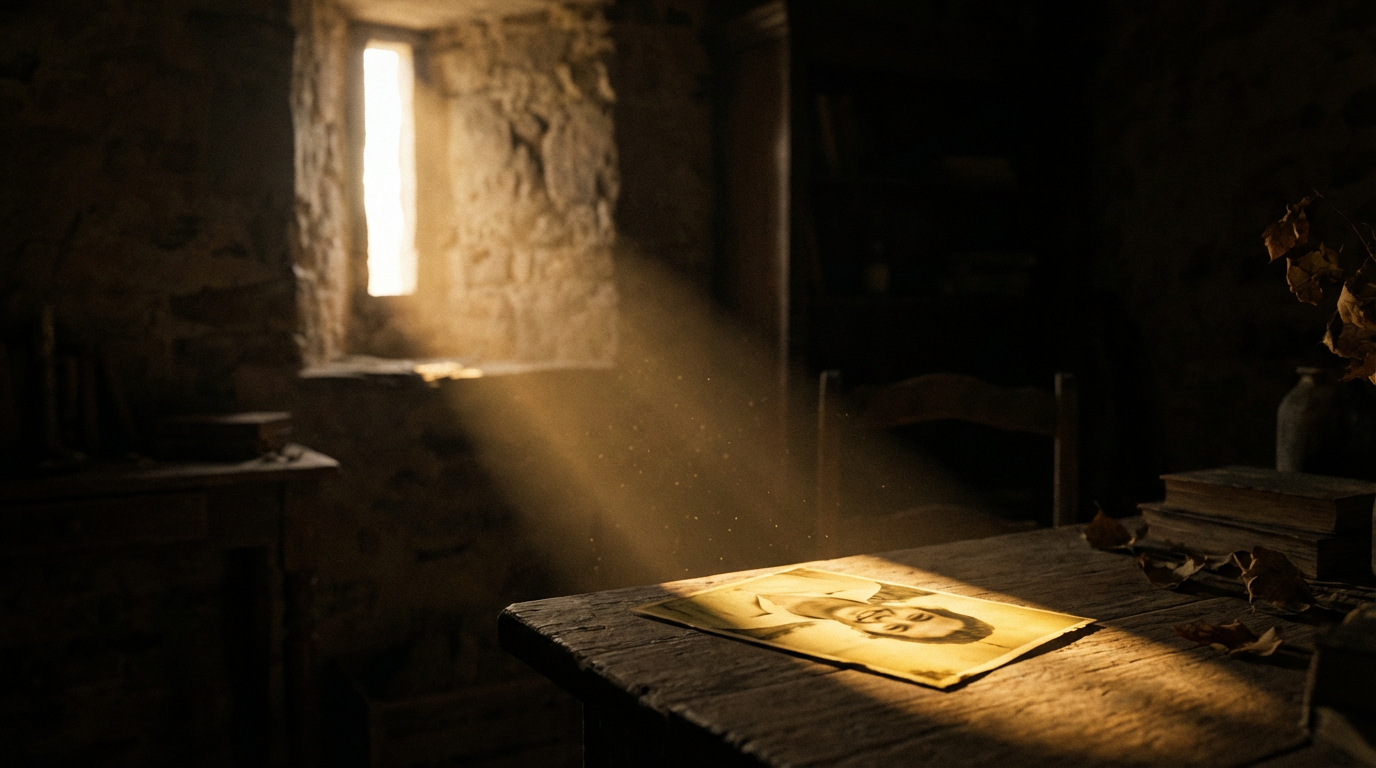
\includegraphics[height=\figheight]{Fig6-1.png}
\caption{Light revealing photograph in darkness—memory and solitude compressed into 1.5 seconds \\ \authorcreated}
\label{fig:light-photo}
\index{figure!compressed narrative}
\end{figure}

\textbf{Psychological Principles:}

\begin{enumerate}
\item Emotion precedes reason—first feel, then understand \citep{kahneman2011thinking}.
\item Rhythm drives perception—each beat influences audience heart rate \citep{kovarski2022movie}.
\item Suggestion surpasses explanation—negative space invites audience co-creation \citep{arnheim1974art}.
\end{enumerate}

\section{The Three-Beat Structure Extended: The Breathing System}
\label{sec:three-beat-structure}
\index{three-beat structure}
\index{breathing system}

Traditional cinema follows ``three-act structure,'' but in micro-narrative, it's compressed into ``three-beat rhythm'': \textbf{Setup—Pulse—Echo}\index{setup-pulse-echo}.

However, truly mature short scenes often have a \textbf{four-layer breathing structure}\index{four-layer breathing}:

\begin{enumerate}
\item \textbf{Setup (0--1.5s)}\index{setup}: Establish environment and emotional baseline. Can use color temperature, tone, spatial lighting to build world sense.

\item \textbf{Pulse (1.5--4s)}\index{pulse}: Emotional or event pulsation. Usually triggered by sudden action, sound, or visual contrast creating a turning point.

\item \textbf{Pause (4--6s)}\index{pause}: Brief stillness allowing audiences to absorb and resonate. Slow motion, reverse shots, or breathing sounds can create psychological suspension.

\item \textbf{Echo (6--8s)}\index{echo}: Lingering moment where emotion transforms into symbol. Can be achieved through light changes, natural elements, or camera movement.
\end{enumerate}

\textbf{Example:}

\begin{Prompt}
A raindrop falls (setup); camera tracks its descent (pulse); dust rises (pause); the ground cracks, a green sprout breaks through the soil (echo).

Nature's rhythm is emotion's rhythm. In these seconds, audiences experience the emergence of ``hope.''
\end{Prompt}

\begin{figure}[H]
\centering
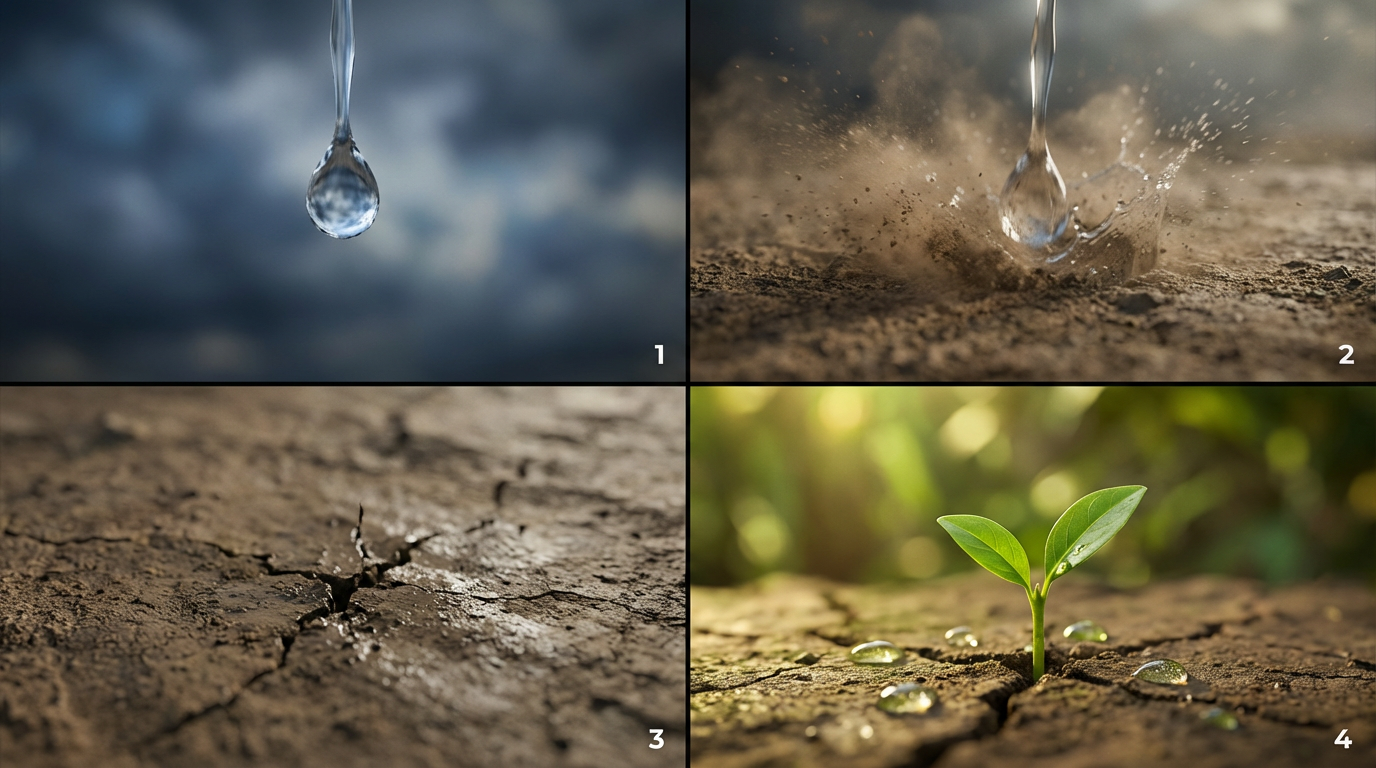
\includegraphics[height=\figheight]{Fig6-2.png}
\caption{Raindrop to sprout—hope emerging through natural rhythm \\ \authorcreated}
\label{fig:raindrop-sprout}
\index{figure!natural symbolism}
\end{figure}

\textbf{Extended Techniques:}

\begin{itemize}
\item Combine sound rhythm with visual rhythm to form ``breathing cadence.''\index{breathing cadence}
\item Use visual repetition to create rhythm, such as flickering lights, dripping rain.
\item Leave ``breathing space'' in the final second, allowing delayed emotional resonance.
\end{itemize}

\section{The Philosophy of Visual Compression: Visual Economy and High-Impact Imagery}
\label{sec:visual-compression}
\index{visual compression}
\index{information density}

Micro-narrative demands imagery with high information density. Every object, every light ray, every angle must serve emotion.

\subsection{Imbuing Objects with Emotion}
\index{objects!as emotional carriers}

In feature films, actors' performances bear emotional expression; in short films, \textbf{objects} become emotional spokespersons. Shattered glass symbolizes regret, a still clock symbolizes frozen time, an empty cup represents an absent relationship. These symbols are the core foundation Sora 2 understands and generates. From practical experience with AI-generated content, we can observe how visual elements unlock emotional responses, enabling the systematic use of symbolic imagery in narrative construction.

\subsection{Metaphorical Logic in Composition}
\index{composition!metaphorical}

Sora 2 can express psychological relationships through compositional structure:

\begin{itemize}
\item Low-angle upward shot → indicates power and the unknown
\item Centered composition → expresses stability and solitude
\item Broken symmetry → suggests conflict
\item Spatial depth → symbolizes distance and time
\end{itemize}

\subsection{Emotional Control Through Light and Color}
\index{light!as emotional language}
\index{color temperature}

Light is the language of time; color is the tonality of emotion.

Cool blue symbolizes loneliness and memory; warm orange represents warmth and hope; extreme contrast lighting creates suspense or fantasy.

\textbf{Example:}

\begin{Prompt}
Warm orange lamplight illuminates a cold metal table; no human figure is visible, yet emotion arrives.
\end{Prompt}

\begin{figure}[H]
\centering

\includegraphics[height=\figheight]{Fig6-3.png}
\caption{Warm light on cold metal—emotion conveyed through contrast alone \\ \authorcreated}
\label{fig:light-contrast}
\index{figure!emotional lighting}
\end{figure}

In just one frame, Sora 2 completes the transmission of ``emptiness'' as feeling.

\subsection{Reuse of Visual Symbols}
\index{visual symbols!recurring}

Recurring imagery can create ``psychological continuity''\index{psychological continuity}—balloons, windows, light spots, shadows can all become ``vocabulary'' of visual language. When audiences see it the second time, they automatically recall the emotion from the first appearance. From our creative practice with AI-generated content, we observe how recurring symbolic elements can build meaning structures and emotional connections across narrative sequences.

\section{Sculpting Time: Rhythm, Pause, and Beat}
\label{sec:sculpting-time}
\index{rhythm design}
\index{temporal sculpting}

Time in imagery doesn't flow objectively but is ``shaped'' by the director. Rhythm design is manipulating audience heart rate. An excellent micro-narrative short film should resemble a miniature symphony.

\begin{table}[H]
\centering
\caption{Rhythm types and their emotional meanings \\ \authorillustration}
\label{tab:rhythm-types}
\index{table!rhythm types}
\small
\begin{tabular}{p{4cm}p{5cm}p{5cm}}
\hline
\textbf{Rhythm Type} & \textbf{Emotional Meaning} & \textbf{Common Use} \\
\hline
Fast cuts (0.5s) & Tight rhythm, strong reaction & Action, thriller, tech ads \\
Medium flow (1--2s) & Stable, natural, daily & Life documentation, brand films \\
Slow contemplation (3--4s) & Meditative, nostalgic, dreamlike & Emotional shorts, art videos \\
\hline
\end{tabular}
\end{table}

\textbf{Golden Rhythm Formula:}\index{golden rhythm formula} Fast → Slow → Stop → Return.

Example:

\begin{Prompt}
She runs (fast); stumbles (fast); looks up to see the sunset (slow); freezes in a smile (stop).
\end{Prompt}

\begin{figure}[H]
\centering
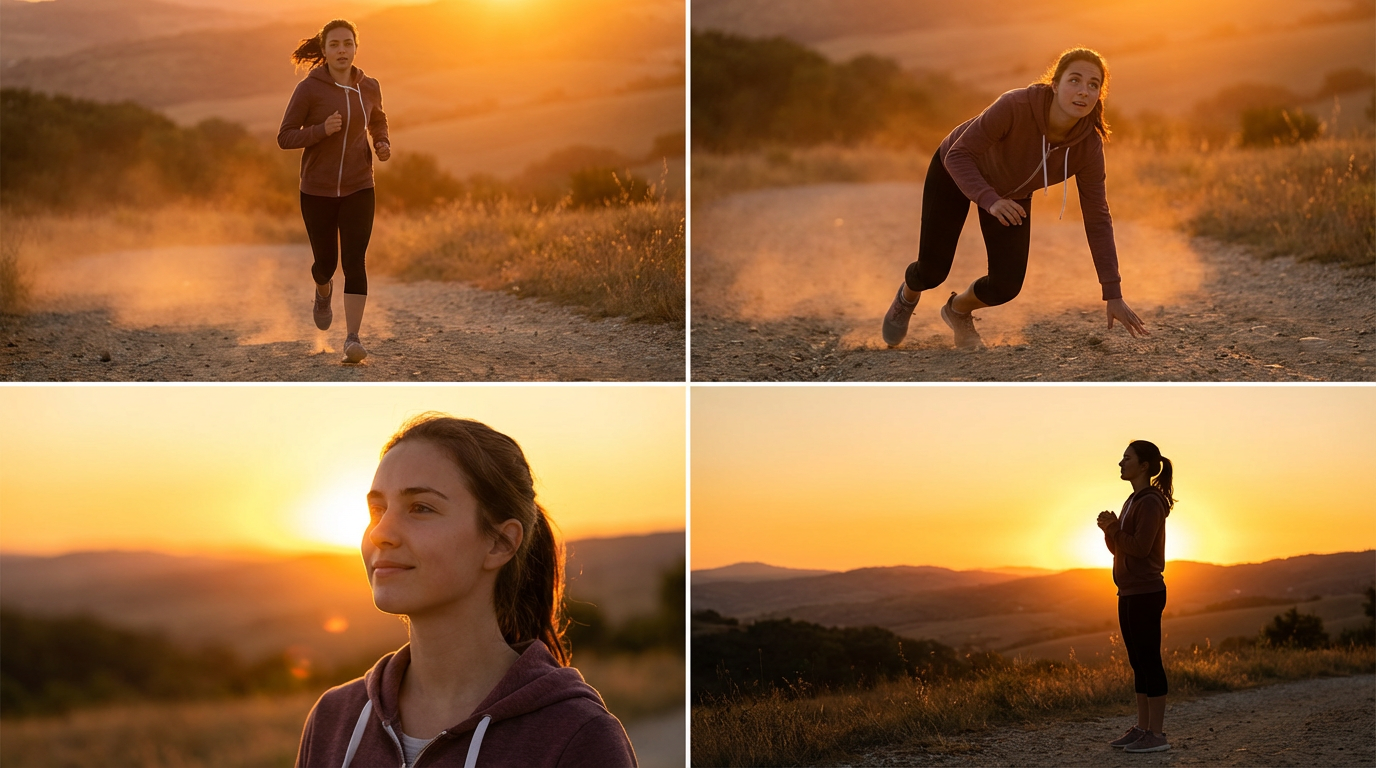
\includegraphics[height=\figheight]{Fig6-4.png}
\caption{Running to stillness—rhythm controlling emotional arc \\ \authorcreated}
\label{fig:rhythm-arc}
\index{figure!rhythmic progression}
\end{figure}

\textbf{Rhythm Techniques:}

\begin{itemize}
\item Use sound-image counterpoint\index{sound-image counterpoint}: sound arrives first, image follows.
\item Utilize ``blank frames''\index{blank frames} to create psychological pauses.
\item Off-beat rhythm creates surprise and memorable moments.
\end{itemize}

\section{The Art of Invisible Transitions}
\label{sec:invisible-transitions}
\index{transitions}
\index{emotional bridges}

In micro-narrative, shot connections determine flow. Transitions are no longer merely technical but ``emotional bridges.''\index{emotional bridges}

\textbf{Main Types:}

\begin{enumerate}
\item \textbf{Action transition}\index{action transition}: Shots connected by consistent action direction, like ``looking up → sky → airplane passing.''

\item \textbf{Light transition}\index{light transition}: Brightness changes bring out emotion, like ``lightning → white field → sunrise.''

\item \textbf{Gaze transition}\index{gaze transition}: Character's gaze guides camera movement, making narrative coherent.

\item \textbf{Color transition}\index{color transition}: Transitioning using the same hue or color system, reinforcing symbolism.
\end{enumerate}

\textbf{Extended Usage:}

\begin{itemize}
\item Achieve ``cross-shot connection'' through sound, like a single breath extending across multiple scenes.
\item Use motion blur and movement trajectories to create ``dreamlike sliding.''\index{dreamlike sliding}
\end{itemize}

\textbf{Example:}

\begin{Prompt}
A boy looks up at fireworks; white flash transition. Next shot: morning light through the window, he wakes in bed. The alternation of night and day symbolizes the connection between dream and reality.
\end{Prompt}

\begin{figure}[H]
\centering
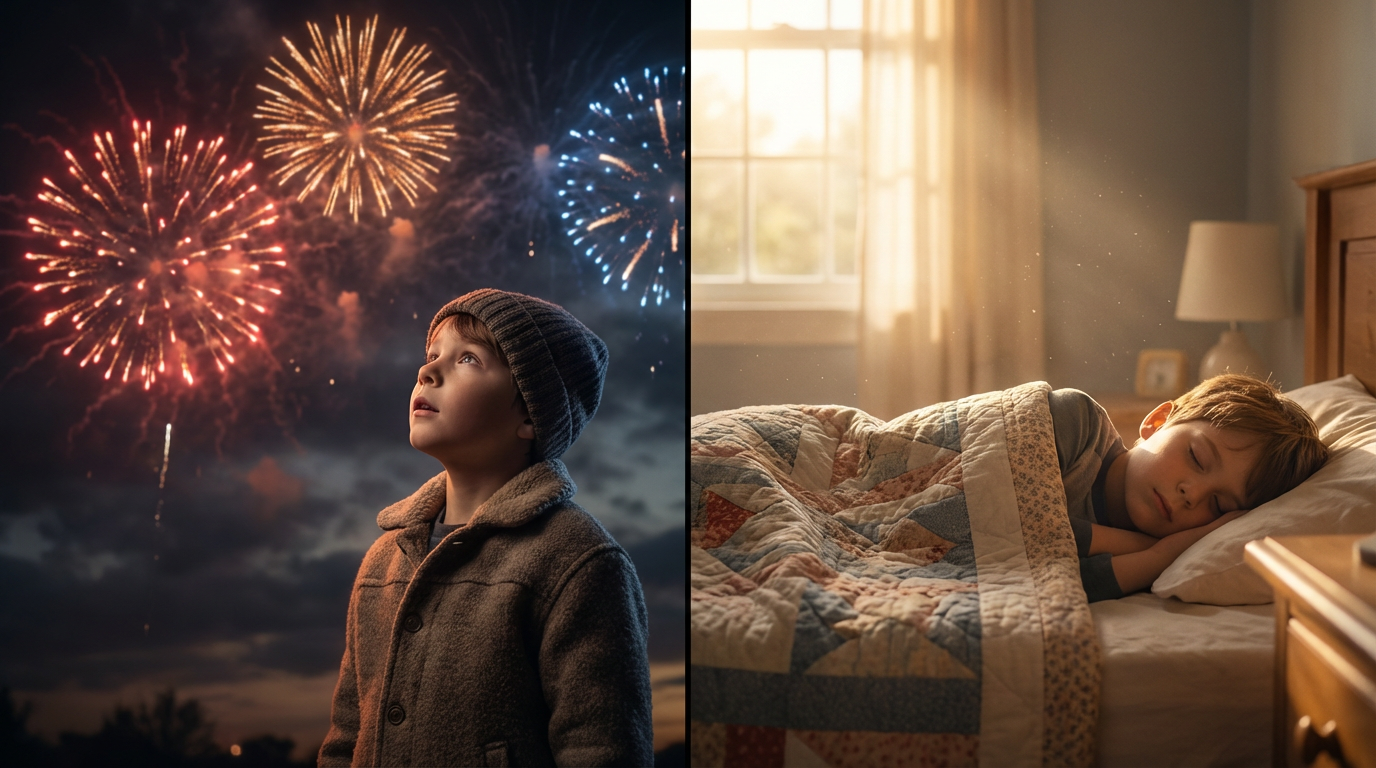
\includegraphics[height=\figheight]{Fig6-5.png}
\caption{Fireworks to morning light—night and day transition through white flash \\ \authorcreated}
\label{fig:dream-reality-transition}
\index{figure!temporal transition}
\end{figure}

\section{The Art of Controlling Tension and Release}
\label{sec:tension-release}
\index{tension}
\index{release}
\index{suspense}

Tension is the foundation of effective short films. Creating suspense within 6 seconds hinges on ``delayed gratification.''\index{delayed gratification}

\begin{itemize}
\item \textbf{Suspended unresolved}\index{suspended moment}: Stop action one frame before the crucial moment. Audience imagination completes the narrative.

\item \textbf{Information gap}\index{information gap}: Deliberately omit cause or effect, prompting active search for answers.

\item \textbf{Sound preceding image}\index{sound-first technique}: Give sound first, then image, triggering instinctive alertness.
\end{itemize}

\textbf{Example:}

\begin{Prompt}
In darkness, water drips. Lights flicker. A hand reaches for the switch—pause—black.
\end{Prompt}

\begin{figure}[H]
\centering
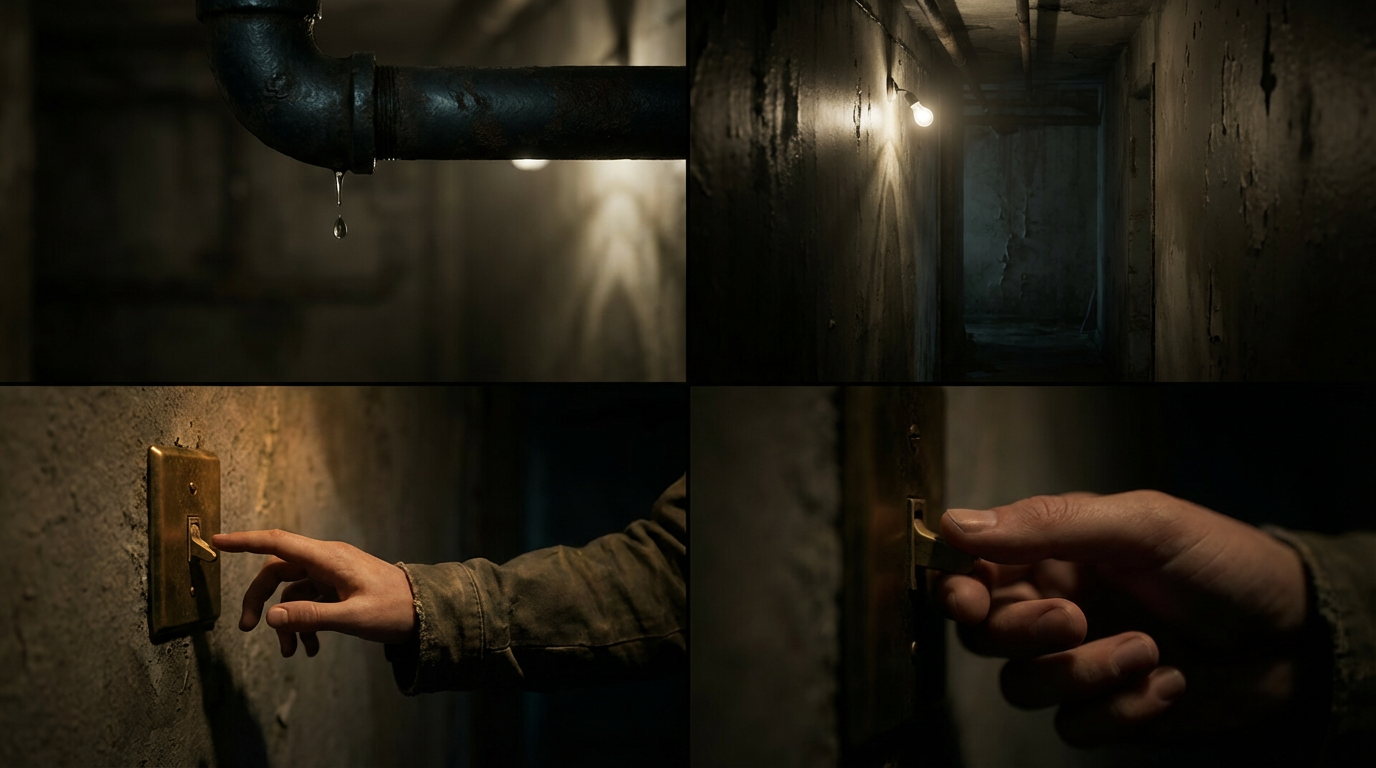
\includegraphics[height=\figheight]{Fig6-6.png}
\caption{Hand reaching for switch in darkness—suspended tension \\ \authorcreated}
\label{fig:suspense-hand}
\index{figure!suspense creation}
\end{figure}

These seconds of suspense suffice to elevate heart rate. The ``stillness'' after tension is the audience's emotional reverberation period. Sora 2 can achieve this emotional release through gradual light extinction, image defocus, or slow pull shots.

\section{Visual Symbolism: Creating Emotional Impact Through Imagery}
\label{sec:visual-poetry}
\index{visual poetry}
\index{poetic cinema}

Advanced short scenes function as visual symbolism\index{visual symbolism}—a structured imagery language composed of rhythm, symbolic elements, and strategic negative space.

\textbf{Core Characteristics:}

\begin{enumerate}
\item \textbf{Symbolism}\index{symbolism}: Objects are embodiments of emotion.
\item \textbf{Rhythmicity}\index{rhythmicity}: Repetition and breathing form visual melody.
\item \textbf{Contrast}\index{contrast}: Interweaving of cold and warm, fast and slow, life and death.
\item \textbf{Negative Space}\index{negative space}: Information withheld from the frame becomes more powerful.
\end{enumerate}

\textbf{Example:}

\begin{Prompt}
A kite's string breaks, ascending into the sky. A child chases in the wind. Camera pulls back; kite disappears. Child stops, smiling upward.
\end{Prompt}

\begin{figure}[H]
\centering
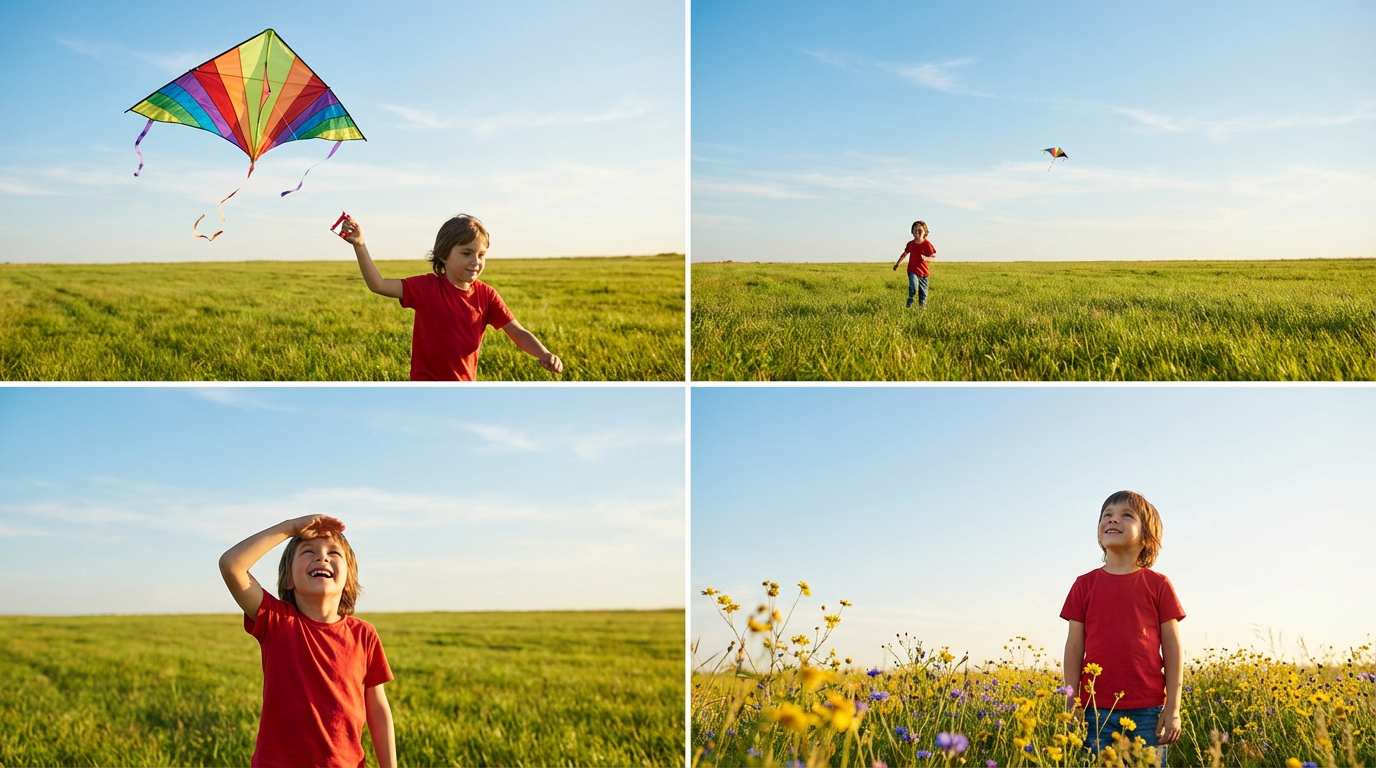
\includegraphics[height=\figheight]{Fig6-7.png}
\caption{Kite ascending—freedom through symbolic imagery \\ \authorcreated}
\label{fig:kite-freedom}
\index{figure!symbolic freedom}
\end{figure}

Sora 2 can understand poetic structure through visual cadence. You can add symbolic words to Prompts, such as ``symbolic wind, lingering gaze, silent echo,'' and AI will express ``artistic conception'' in visual form.

\section{Creative Exercise: Complete Narrative in 8 Seconds}
\label{sec:creative-exercise}
\index{creative exercises}

\textbf{Structural Template:}

\begin{Prompt}
[Atmosphere] + [Action] + [Turning Point] + [Echo]
\end{Prompt}

\textbf{Basic Exercise:}

\begin{Prompt}
Morning kitchen. Young father fries eggs; child hands him salt. Father pauses, smiles and nods. —Family warmth established in 2 seconds.
\end{Prompt}

\textbf{Advanced Challenge:}

Create a ``dual-layer symbolic'' story where literal and metaphorical meanings both hold.

\begin{Prompt}
Girl scatters flower petals on a lake surface. Camera reverses—the lake surface is actually the reflection of a tombstone.
\end{Prompt}

\begin{figure}[H]
\centering
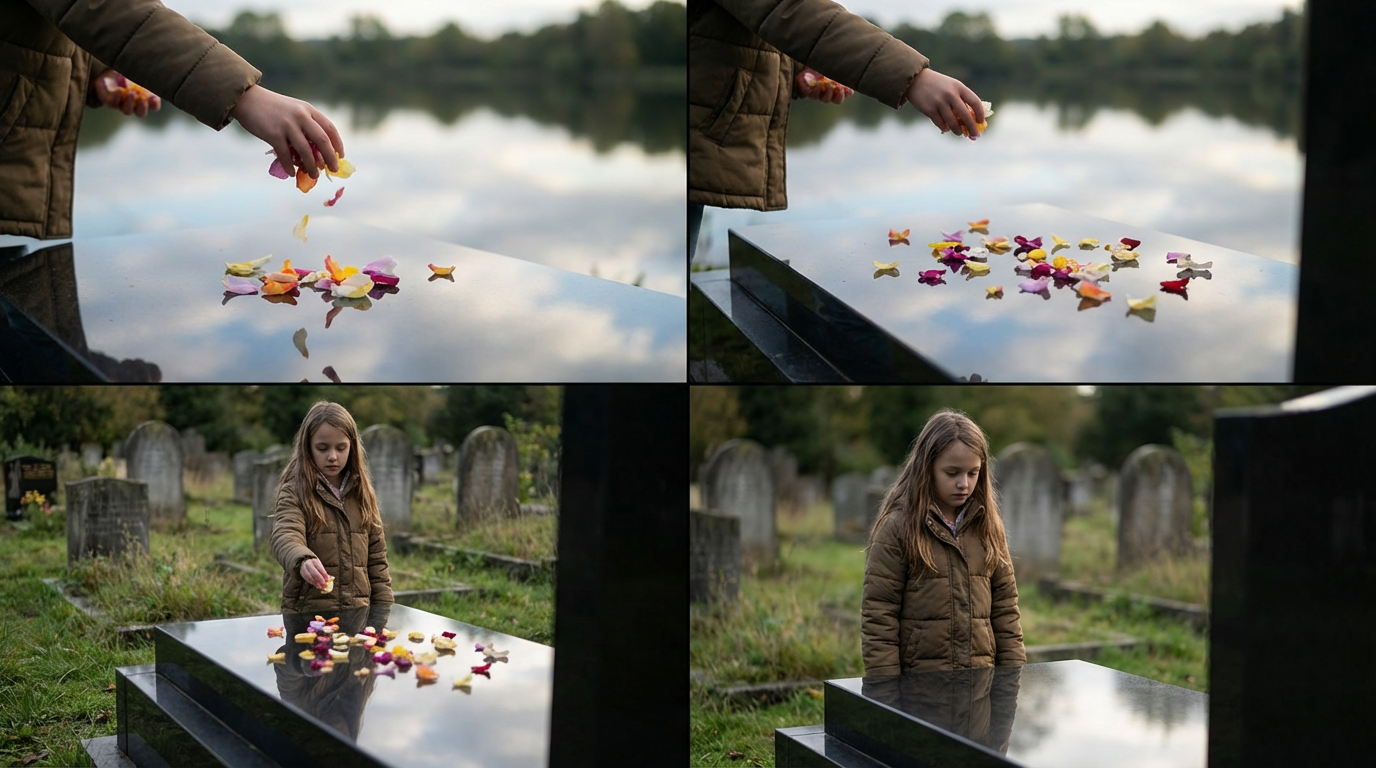
\includegraphics[height=\figheight]{Fig6-8.png}
\caption{Lake reflection revealing tombstone—dual-layer symbolism \\ \authorcreated}
\label{fig:dual-symbolism}
\index{figure!layered meaning}
\end{figure}

\textbf{Extended Training:}

\begin{enumerate}
\item Tell a complete event in one shot.
\item Use a sound to suggest an unseen character.
\item Use color changes to replace dialogue in completing narrative.
\end{enumerate}

\section{Professional Applications: Micro-Narrative Language in Ads, Brands, and MVs}
\label{sec:professional-applications}
\index{commercial applications}
\index{advertising}
\index{brand films}

Micro-narrative is the core capability of modern visual communication. Advertising, branding, public service, MVs, trailers all rely on it for high-density information transmission.

\textbf{Brand Advertising:}

\begin{Prompt}
Woman running in rain, falls and rises. Brand slogan: ``Never Stop.''
\end{Prompt}

\begin{figure}[H]
\centering
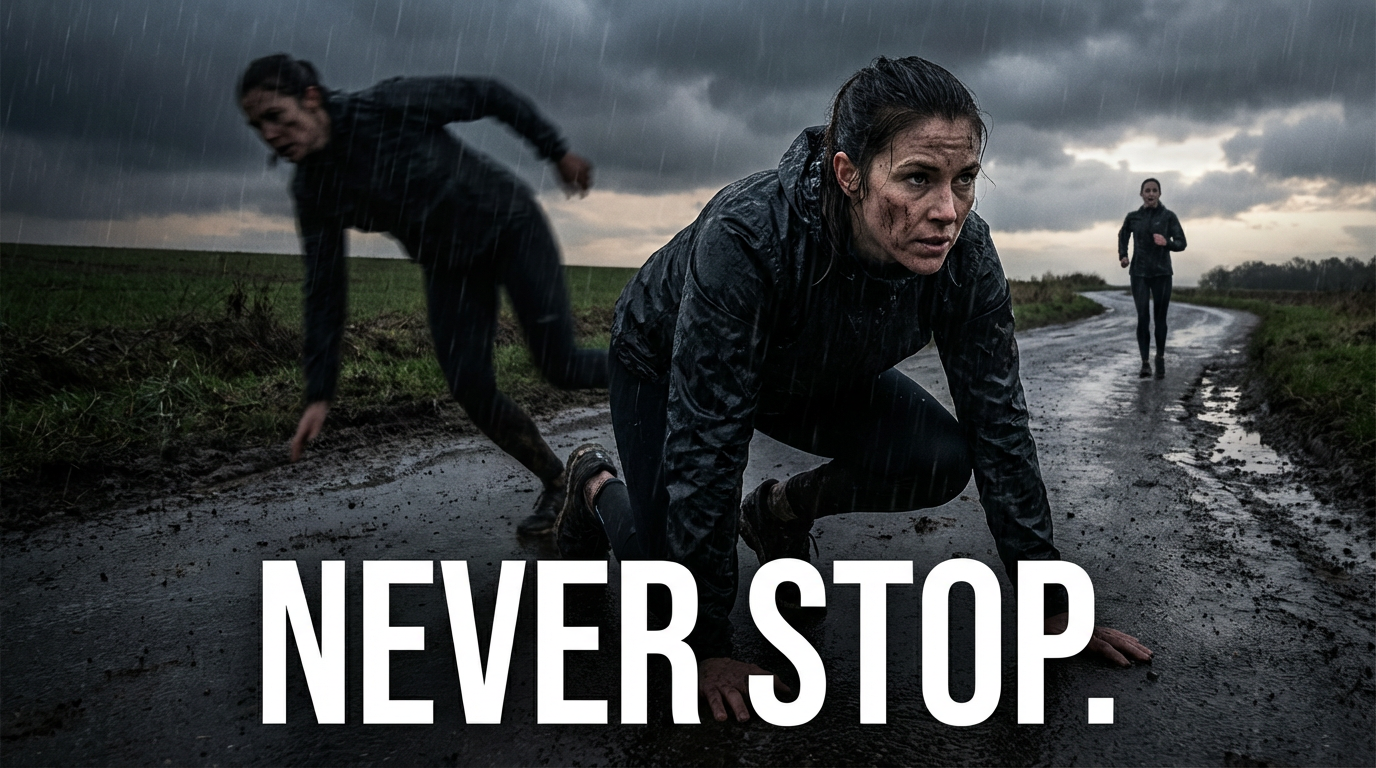
\includegraphics[height=\figheight]{Fig6-9.png}
\caption{Woman rising from fall—brand resilience narrative \\ \authorcreated}
\label{fig:brand-resilience}
\index{figure!brand narrative}
\end{figure}

\textbf{Public Service Short:}

\begin{Prompt}
Breathing sounds in black screen; lights brighten—firefighter removes helmet, sweat dripping.
\end{Prompt}

\begin{figure}[H]
\centering
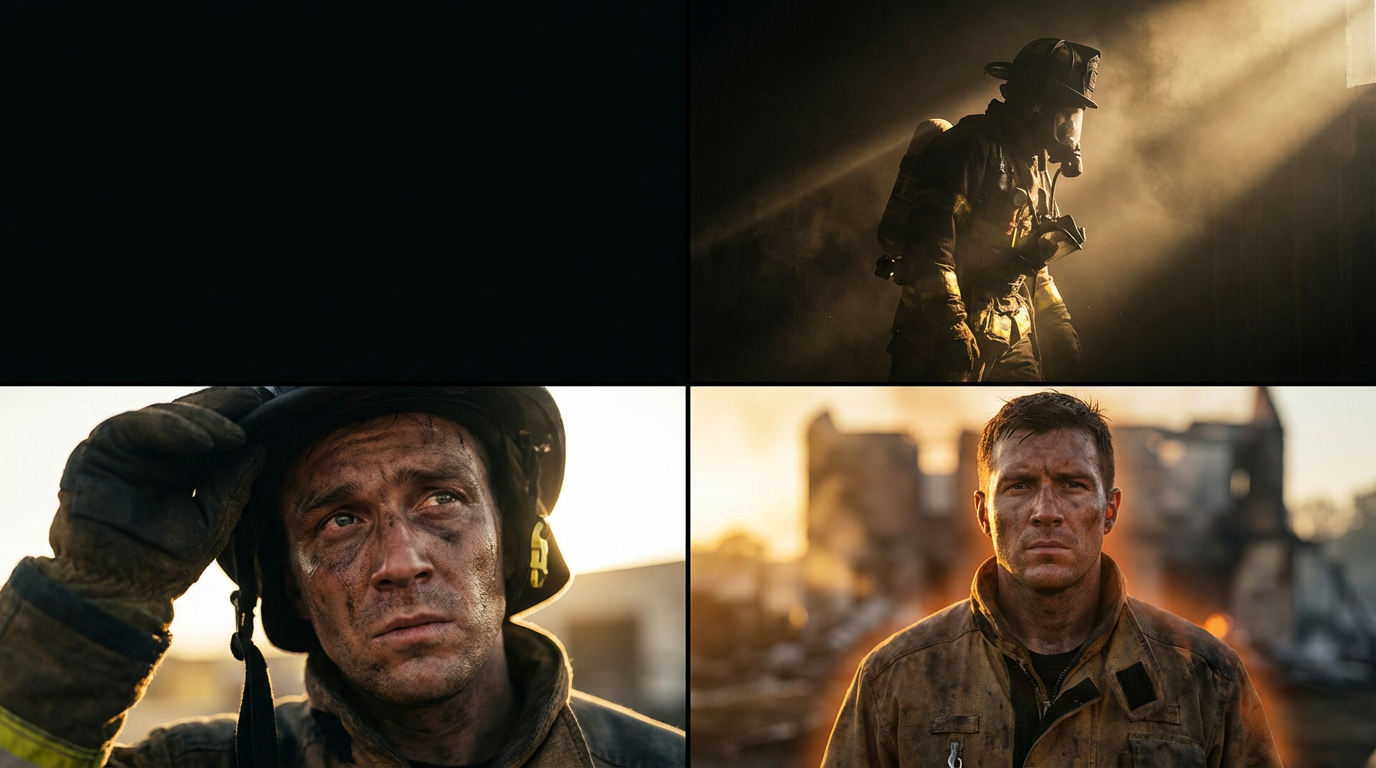
\includegraphics[height=\figheight]{Fig6-10.png}
\caption{Firefighter removing helmet—public service emotional impact \\ \authorcreated}
\label{fig:firefighter}
\index{figure!public service}
\end{figure}

\textbf{Music MV Segment:}

\begin{Prompt}
Rhythm synchronized with emotion; each drumbeat of melody corresponds to the breathing of shots.
\end{Prompt}

When creating Sora 2 Prompts, prioritize describing \textbf{visual emotional curves}\index{visual emotional curve} rather than textual plot. For example:

\begin{Prompt}
``warm sunset through raindrops, girl smiles in reflection''
\end{Prompt}

Far more cinematic than ``girl feels hope after rain.''

\section{Conclusion: Mastering Temporal Narrative Techniques}
\label{sec:short-scenes-conclusion}

Micro-narrative storytelling isn't compression but \textbf{refinement}\index{refinement}. It makes us reconsider the essence of narrative:

\begin{Prompt}
Can a single moment bear true emotion?
\end{Prompt}

The answer is: yes.

A glance, a tear, a beam of light—each element can convey complete emotional meaning. Technical constraints become creative opportunities; brevity enables concentrated impact. Each second represents precise emotional design; each frame carries intentional narrative weight.

Effective 8-second emotional impact demonstrates mastery of compressed storytelling techniques\index{compressed storytelling}.

\section*{Practical Exercises}
\index{practical exercises}

\begin{quote}
\textit{\textbf{Timeless Principle:} Even as interfaces evolve and platforms update, the underlying visual logic---light, composition, rhythm, and emotional resonance---remains eternal. Master these fundamentals, and you will adapt effortlessly to any future tool.}
\end{quote}

\subsection*{Exercise 1: Four-Layer Emotional Arc Construction}
\textbf{Objective}: Master the Inhale → Hold → Exhale → Pause structure for complete emotional storytelling.

\textbf{Progressive Building Exercise}:
\begin{enumerate}
\item \textbf{Inhale (Setup - 2 seconds)}:
   \begin{itemize}
   \item "Elderly man approaches park bench"
   \item "Young woman checks phone nervously"
   \item "Child stares at closed door"
   \end{itemize}
\item \textbf{Hold (Tension - 2-3 seconds)}:
   \begin{itemize}
   \item "Notices worn nameplate on bench"
   \item "Message notification appears"
   \item "Hears laughter from inside"
   \end{itemize}
\item \textbf{Exhale (Release - 2 seconds)}:
   \begin{itemize}
   \item "Gentle smile, touches nameplate"
   \item "Relief spreads across face"
   \item "Knocks confidently"
   \end{itemize}
\item \textbf{Pause (Reflection - 1 second)}:
   \begin{itemize}
   \item "Sits peacefully, looking skyward"
   \item "Puts phone away, walks forward"
   \item "Door opens, warm light spills out"
   \end{itemize}
\end{enumerate}

\textbf{Practice Assignment}: Create four-layer arcs for these emotions:
\begin{itemize}
\item Discovery and wonder
\item Loss and acceptance
\item Fear and courage
\end{itemize}

\subsection*{Exercise 2: Symbolic Visual Language}
\textbf{Objective}: Replace exposition with symbolic imagery that triggers emotional responses.

\textbf{Symbol Translation Practice}:
\begin{itemize}
\item \textbf{Literal}: "She felt lonely" 
\item \textbf{Symbolic}: "Empty chair at dinner table, single place setting"
\item \textbf{Literal}: "He was determined"
\item \textbf{Symbolic}: "Worn running shoes, early morning mist, steady breathing"
\item \textbf{Literal}: "They were in love"
\item \textbf{Symbolic}: "Two coffee cups, steam intertwining, shared newspaper"
\end{itemize}

\textbf{Advanced Symbolism}:
\begin{enumerate}
\item \textbf{Temporal Symbols}: "Clock hands moving backward" (regret/nostalgia)
\item \textbf{Natural Metaphors}: "Flower blooming in fast-forward" (growth/potential)
\item \textbf{Object Transformation}: "Paper airplane becomes real bird" (dreams realized)
\end{enumerate}

\textbf{Practice Challenge}: Create symbolic representations for:
\begin{itemize}
\item Forgiveness
\item Ambition
\item Healing
\item Betrayal
\end{itemize}

\subsection*{Exercise 3: Psychological Timing Mastery}
\textbf{Objective}: Leverage precise timing windows for maximum emotional impact.

\textbf{Timing Framework}:
\begin{itemize}
\item \textbf{0.1-second Recognition}: First visual element must be instantly identifiable
\item \textbf{0.4-second Emotional Response}: Emotional trigger must activate within this window
\item \textbf{2-second Memory Formation}: Complete emotional concept must crystallize
\item \textbf{8-second Total Arc}: Full narrative cycle with resolution
\end{itemize}

\textbf{Precision Timing Exercise}:
\begin{Prompt}
\textbf{0-0.1s}: "Close-up: weathered hands"\\
\textbf{0.1-0.5s}: "Hands trembling slightly"\\
\textbf{0.5-2s}: "Reaching for old photograph"\\
\textbf{2-6s}: "Photograph shows young couple"\\
\textbf{6-8s}: "Gentle smile, tear falls"
\end{Prompt}

\textbf{Practice}: Create precise timing for these scenarios:
\begin{itemize}
\item Moment of realization
\item Unexpected reunion
\item Silent goodbye
\end{itemize}

\section*{Micro-Narrative Templates}
\index{narrative templates}

\subsection*{Template 1: Emotional Revelation}
\begin{Prompt}
\textbf{[Visual Setup]} → [Symbolic Element] → [Emotional Recognition] → [Resonant Conclusion]

Example: "Child's drawing on refrigerator → crayon breaks → child's disappointed face → parent's encouraging hug"
\end{Prompt}

\subsection*{Template 2: Temporal Compression}
\begin{Prompt}
\textbf{[Past Indicator]} → [Present Moment] → [Future Implication] → [Emotional Bridge]

Example: "Wedding ring in jewelry box → woman's hesitant hand → empty finger → determined expression"
\end{Prompt}

\subsection*{Template 3: Symbolic Transformation}
\begin{Prompt}
\textbf{[Initial State]} → [Catalyst Moment] → [Transformation Process] → [New Reality]

Example: "Wilted flower → single water drop → time-lapse blooming → vibrant garden"
\end{Prompt}

\section*{Emotional Impact Checklist}
\index{emotional impact}

\subsection*{Pre-Creation Assessment}
\begin{itemize}
\item[$\square$] \textbf{Core Emotion}: Is the primary emotion clearly defined?
\item[$\square$] \textbf{Visual Clarity}: Can the emotion be understood without dialogue?
\item[$\square$] \textbf{Symbolic Resonance}: Do visual elements carry deeper meaning?
\item[$\square$] \textbf{Timing Precision}: Are emotional beats aligned with psychological windows?
\item[$\square$] \textbf{Universal Appeal}: Will the emotion translate across cultures?
\item[$\square$] \textbf{Memory Trigger}: Does the scene create a lasting emotional impression?
\end{itemize}

\subsection*{Post-Creation Evaluation}
\begin{itemize}
\item[$\square$] \textbf{Immediate Recognition}: Is the emotion instantly identifiable?
\item[$\square$] \textbf{Emotional Authenticity}: Does the emotion feel genuine and earned?
\item[$\square$] \textbf{Visual Efficiency}: Is every element contributing to the emotional goal?
\item[$\square$] \textbf{Narrative Completeness}: Does the scene tell a complete emotional story?
\item[$\square$] \textbf{Lasting Impact}: Does the emotion resonate after viewing?
\end{itemize}

\section*{Common Micro-Narrative Challenges}
\index{troubleshooting}

\begin{table}[H]
\centering
\caption{Micro-Narrative Storytelling Issues and Solutions \\ \authorillustration}
\label{tab:narrative-issues}
\begin{tabular}{p{4cm}p{4cm}p{5cm}}
\hline
\textbf{Issue} & \textbf{Symptom} & \textbf{Solution} \\
\hline
Unclear Emotion & Audience confusion about intended feeling & Strengthen symbolic elements, simplify visual metaphors \\
\hline
Rushed Pacing & Emotional beats feel hurried & Extend key moments, allow for emotional processing time \\
\hline
Over-Symbolism & Meaning becomes obscure & Balance symbolic and literal elements, test with diverse viewers \\
\hline
Weak Resolution & Emotional arc feels incomplete & Strengthen the "Pause" phase, ensure clear emotional conclusion \\
\hline
Cultural Disconnect & Symbols don't translate universally & Use more universal human experiences, avoid culture-specific references \\
\hline
\end{tabular}
\end{table}

\section*{Advanced Micro-Narrative Techniques}
\index{advanced techniques}

\subsection*{Technique 1: Layered Symbolism}
Create multiple levels of meaning within single images:
\begin{Prompt}
"Rain on window → tears on face → cleansing/renewal → new beginning"
\end{Prompt}

\subsection*{Technique 2: Emotional Counterpoint}
Contrast visual and emotional elements for deeper impact:
\begin{Prompt}
"Bright carnival lights → child's sad expression → isolation in crowds"
\end{Prompt}

\subsection*{Technique 3: Temporal Echoing}
Use visual callbacks to create emotional resonance:
\begin{Prompt}
"Empty swing moving → flashback to child playing → present: parent watching → future: hope"
\end{Prompt}

\section*{Professional Application Framework}
\index{professional applications}

\subsection*{Brand Storytelling Applications}
\begin{itemize}
\item \textbf{Product Launch}: Use transformation symbolism to show before/after states
\item \textbf{Brand Values}: Embed company principles in visual metaphors
\item \textbf{Emotional Branding}: Create instant emotional connections through symbolic imagery
\end{itemize}

\subsection*{Social Media Optimization}
\begin{itemize}
\item \textbf{Platform-Specific Timing}: Adjust emotional pacing for Instagram (3-5s) vs TikTok (8-15s)
\item \textbf{Scroll-Stopping Power}: Front-load emotional impact in first 0.5 seconds
\item \textbf{Shareability Factor}: Create emotionally resonant moments that encourage sharing
\end{itemize}

\section*{Chapter Summary}

Key actionable insights for micro-narrative storytelling:

\begin{itemize}
\item \textbf{Psychological Timing}: Leverage the 0.1-second recognition, 0.4-second emotional response, and 2-second memory formation windows
\item \textbf{Four-Layer Structure}: Use Inhale (setup) → Hold (tension) → Exhale (release) → Pause (reflection) for complete emotional arcs
\item \textbf{Visual Symbolism}: Replace exposition with symbolic imagery that triggers subconscious emotional responses
\item \textbf{Rhythm Synchronization}: Match visual pacing to intended emotional beats and platform-specific attention patterns
\item \textbf{Compression Techniques}: Focus on visual emotional curves rather than plot exposition for maximum impact in minimal time
\end{itemize}
